\documentclass[12pt,final,a4paper,oneside]{book}
\usepackage{lmodern,graphicx,longtable,enumerate,tabularx,booktabs,amsmath,suffix,xspace,xcolor}
\usepackage{hyperref,booktabs}
\usepackage[ngerman,english]{babel}
\usepackage[utf8]{inputenc}
\usepackage[T1]{fontenc}
\usepackage[longnamesfirst]{natbib}

\usepackage{lipsum}

% This defines the chapter authors
\newcommand\chapterauthor[1]{\authortoc{#1}\printchapterauthor{#1}}
\WithSuffix\newcommand\chapterauthor*[1]{\printchapterauthor{#1}}

\makeatletter
\newcommand{\printchapterauthor}[1]{%
	{\parindent0pt\vspace*{-25pt}%
		\linespread{1.1}\large\scshape#1%
		\par\nobreak\vspace*{35pt}}
	\@afterheading%
}
\newcommand{\authortoc}[1]{%
	\addtocontents{toc}{\vskip-10pt}%
	\addtocontents{toc}{%
		\protect\contentsline{chapter}%
		{\hskip1.3em\mdseries\scshape\protect\scriptsize#1}{}{}}
	\addtocontents{toc}{\vskip5pt}%
}
\makeatother

% define environment for the abstract:
%   Generate the environment for the abstract:
\newenvironment{abstract}
{ \paragraph*{Summary} }
{ \bigskip}

\newenvironment{goals}
{ \noindent  \paragraph*{Learning Objectives} \begin{itemize}}
	{ \end{itemize}\bigskip}	


\newenvironment{testquestion}
{ \noindent   \section{Test Questions} \begin{itemize}}
	{ \end{itemize}}	

\newenvironment{glossy}
{ \noindent   \section{Glossary} \begin{description}}
	{ \end{description}}	


% Define the R-Logo
\definecolor{Rcolor}{RGB}{150,160,190}

\newcommand{\R}{%
	\raisebox{.3em}{\hspace{1.2em}%
		\llap{\resizebox{1.09em}{.5em}{\color{black}$\bigcirc$}}%
		\llap{\resizebox{1.199em}{.55em}{\color{darkgray}$\bigcirc$}}%
		\llap{\resizebox{1.19em}{.52em}{\color{gray!50}$\bigcirc$}}%
		\llap{\resizebox{1.1em}{.5em}{\color{gray}$\bigcirc$}}%
		\llap{\resizebox{1.25em}{.55em}{\color{gray}$\bigcirc$}}%
	}%
	\hspace{-.85em}%
	\textbf{%
		\textcolor{black}{\textsf{R}}%
		\hspace{-.025em}\raisebox{.01em}{\llap{\textcolor{Rcolor}{\textsf{R}}}}%
	}%
	\xspace}

\pagestyle{plain}
%%%%%%%%%%%%%%%%%%%%%%%%%%%%%%%%%%%%%%%%%%%%%%%%%%%%%%%%%%%%%%%%%

\begin{document}
	
	\title{Project Work in Data Science for Business}
	\author{Dr. Stephan Huber\thanks{stephan.huber@hs-fresenius.de} (Module Coordinator)
		\and your name (Student)
		\and Michael Jackson (Student)
		\and Bob Ross (Student)
	}
	\date{\today}
	\maketitle
	\thispagestyle{empty}
	\newpage
	
	\chapter*{Preface}
	This document should help to describes and paraphrases how the project work in the course \textit{Data Science for Business} should look like. The paper is structured as follows: Chapter \ref{ch:sketch} gives an idea of how the project paper can be structured. In \autoref{ch:listoftopics} the titles of the projects are listed and \autoref{ch:procedure} offers a brief outlook.
	
	Overall, the idea of the project is that we write a textbook together that can work as an applied introduction to data science for students of business administration. Each project consists of one chapter. Of course, students can work together, form groups, and divide work with respect their preferences and talents, respectively. However, every student is responsible (and is graded) for his/her chapter and his/her presentation only. 
	
	Moreover, I will implement (and monitor) your working process using GitHub. I will explain you how that works in a video. 
	
	Please notice, that this document is not written to be self-explaining. It should rather work as a template. I explain everything in further detail during a GoToMeeting. 
	
	
	\tableofcontents
	\listoftables
	\listoffigures
	
	\chapter{A Sketch of How a Project Should Look Like}\label{ch:sketch}
	\chapterauthor{Barbara Streisand \\ barbara@email.de}
	
	\begin{abstract}
		This chapter offers a sketch on how a project may be structured. A project should include a summary, learning objectives, a motivation, a methodolocigal section, a section with an application in \R, an example from businesses, a conclusion, exercises, test questions, and a glossary.\\ 
		\textit{An abstract should make clear in simple language what the chapter is all about. Its maximum length is 200 words.} 
	\end{abstract}
	
	\begin{goals}
		\item ;weruhkltewiouthb
		\item swdfgwserg
	\end{goals}
	
	
	\section{Motivation}
	Motivate your topic. Discuss why the topic and the content of your chapter may be of importance for the reader. Make the content of your chapter subject of a discussion. Outline clearly what the reader can expect. Include a description of contents. For example, write at the end of this section ``The remainder of the chapter is structured as follows: Section 1.2 introduces the theory...''. Additionally, mention which related topics will not be discussed. Recommend literature for self-study here.\footnote{Making a footnote or citing in \LaTeX\ is easy. For example, \citet[see][p. XY]{Provost2013Data} or \citep{Provost2013Data}}
	
	\section{Methodological Issues}
	Bring the statistical theory or econometric approach to the reader. Try to raise a basic understanding of the meaning and the difficulties of the respective method. 
	
	\section{Applications in R}\label{sec:applicationsinR}
	Explain how your topic can be addressed by using \R and RStudio, respectively. In particular, introduce \R-packages that allow to implement the respective methods. Offer a \R-script that allows the reader to understand both the method and the programming skills that are needed to apply the method. It should be possible for the reader to replicate the stuff that is presented in the section and the script.
	
	\section{Example(s) From the Real World}\label{sec:examplerealworld}
	Make an impressive\footnote{The example should be a significant academic contribution, i.e., the example is published in a highly ranked academic journal. Alternatively, the economic impact of the example should be sizable.} example from the \textit{real world} to deepen the application and the methods discussed above. The example can stem either from the \textit{academic world} or the \textit{business world}. For example, pick an \textit{academic} research paper and summarize it to the reader in a way that he can understand the strengths and weaknesses of the respective investigation. Or, you can explain a business case where the method of interest plays an important role to solve a problem or to earn money, for example. 
	
	Sections \ref{sec:applicationsinR} and \ref{sec:examplerealworld} can be combined.
	
	\section{Conclusion}
	Conclude the chapter. This may include a short summary, an outlook and/or related literature.
	
	\section{Exercises}
	\begin{enumerate}[(1)]
		\item Design an exercise that helps the reader to understand and repeat important concepts.
		\begin{enumerate}[a)]
			\item Challenge the reader to think about the topic.
			\item Encourage a discussion.
			\item Bring up new aspects of the method.
			\item Be creative.
		\end{enumerate}
	\end{enumerate}
	
	
	\begin{testquestion}
		\item Ask five short test questions that refer to five important insights from your chapter. A discerning reader should have no problems with these questions.
	\end{testquestion}
	
	\begin{glossy}
		\item[word] This text should define the meaning of word.
	\end{glossy}
	
	
	\chapter{List of Topics}\label{ch:listoftopics}
	\chapterauthor{Michael Jackson\\ mj@king.com}
	
	\begin{abstract}
		Read the following titles of potential projects and send me an email with three topics  you could image working on (\url{stephan.huber@hs-fresenius.de}). Rank them according to your preferences. I will try to consider your wishes.  
		Feel free to make your own suggestions. But please, don't forget to name overall three (!) topics. If everybody likes to have the same topic, I flip a coin and/or try to consider your second and third preference. 
	\end{abstract}
	
	\begin{enumerate}
		
		\item{Data Collection in Data Science}
		
		\item{Exploratory Data Analysis in Data Science}
		%Data scientist can tell a story with data. Introduce a selection of methods that can help to find and \textit{tell a story} with data.
		
		\item{Regression Analysis in Data Science}
		
		\item{Spatial Analysis in Data Science}
		
		\item{Nearest Neighbor Analysis in Data Science}
		
		\item{Decision Trees Analysis in Data Science}
		
		\item{Text Mining Analysis in Data Science}
		
		\item{Big Data Analysis in Data Science}
		
		\item{Machine Learning in Data Science}
		
		\item{Single-Board Computers in Data Science}
		
	\end{enumerate}
	
	
	\chapter{Further Procedure}\label{ch:procedure}
	\chapterauthor{Bob Ross\\ goodnight@paint.org}
	
	The project work includes the following:
	\begin{itemize}
		\item Write a chapter on you topic as paraphrased above. Length of the paper should be about 25 pages.
		\item Prepare a presentation of 20 minutes length (we will see how we manage that part).
		\item Use the Latex to write the chapter.
		\item Use Github to include your chapter into the book which contains all chapters.
		\item Use R and upload your R-code to Github.
	\end{itemize}
	
	\section{\LaTeX}
	
	\LaTeX\ is easy and powerful. It allows the author to focus on the content because he don't need to take care about the layout very much. There are millions of sources online that provide tutorials. You can include figures in an floating environment\footnote{The placement of the figure is optimized automatically.}, see \autoref{fig:td}. Tables are possible, too. See \autoref{tab:tabex} or you can reference online sources, see \url{https://texdoc.net/texmf-dist/doc/latex/booktabs/booktabs.pdf} for a guide to make nice tables.
	
	\begin{figure}\centering
		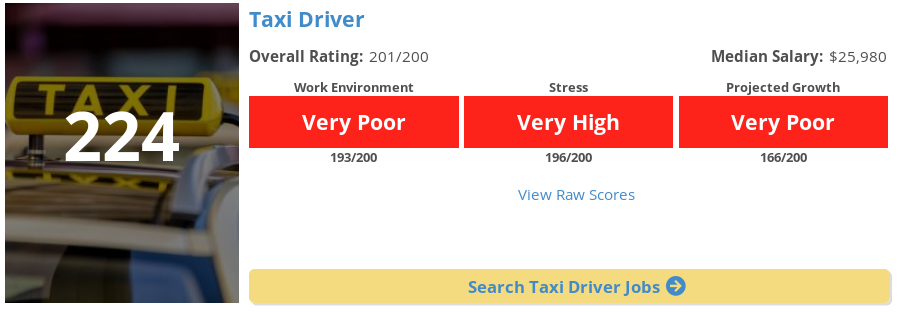
\includegraphics[width=0.5\linewidth]{pic/td}\caption{This is a picture}\label{fig:td}
	\end{figure}
	
	\begin{table}\centering
		\caption{This is a table}\label{tab:tabex}
		\begin{tabular}{@{}llr@{}} \toprule\multicolumn{2}{c}{Item} \\ \cmidrule(r){1-2}Animal & Description & Price (\$)\\ \midrule Gnat  & per gram  & 13.65 \\& each      & 0.01 \\Gnu   & stuffed   & 92.50 \\Emu   & stuffed   & 33.33 \\Armadillo & frozen & 8.99 \\ \bottomrule
		\end{tabular}
	\end{table}
	
	\section{Git and GitHub}
	GitHub  provides hosting for software development version control using Git which is a version control system designed to handle projects with many contributors. Both tools are heavily used in software engineering and data science. It is particularly powerful when teams work on projects with a procedural workflow.
	
	\section{Style of Writing}
	Assume your reader is a well informed master student of business administration. Make things easy for your reader. Believe me, this sounds so easy but it is actually the most difficult task for scientists and academic writers. I got a lot out of reading  \textit{Writing Tips for Ph.  D. Students} from \cite{Cochrane2005Writing}\footnote{You can download this file using \url{https://t1p.de/br5o}}. While you are not a Ph. D. student, these writing tips apply for all authors who aim to communicate efficiently. 
	
		\chapter{Topic 1}\label{ch:topic1}
	\chapterauthor{Student \\ student@email.de}
	
	\begin{abstract}
		This is my abstract.
	\end{abstract}
	
	\begin{goals}
		\item ;
	\end{goals}
	
	\section{Motivation}

	\section{Methodological Issues}

	\section{Applications in R}\label{sec:applicationsinR}

	\section{Example(s) From the Real World}\label{sec:examplerealworld}

	\section{Conclusion}

	\section{Exercises}
	\begin{enumerate}[(1)]
		\item Design 
		\begin{enumerate}[a)]
			\item C
		\end{enumerate}
	\end{enumerate}
	
	
	\begin{testquestion}
		\item A
	\end{testquestion}
	
	\begin{glossy}
		\item[w] T
	\end{glossy}
	
	
	\bibliographystyle{aer}
	\bibliography{lit}
	
\end{document} 
